\chapter{Motivación y Contexto}

Durante los últimos años distintas áreas de la industria han mostrado interés en la fotónica por el elevado ancho de banda que ofrece en comunicaciones.
Sin darnos cuenta, esta tecnología se ha ido integrando a nuestro día a día comenzando con el éxito de los cables ópticos.
Probablemente, la creciente popularidad de esta área es debido a que el siguiente paso lógico para mejorar el rendimiento de los dispositivos electrónicos, los cuales están llegando a sus límites físicos, parece ser la incorporación o acondicionamiento de estos con dispositivos fotónicos \citep{Glick2018, LukasChrostowski2010}.
Sin embargo, la convergencia de estas tecnologías aún presenta muchos desafíos. Particularmente, existen dispositivos como el \emph{bend-90°} y \emph{2-splitter} que aún no logran aplicación industrial aún cuando son fundamentales para una variedad de circuitos fotónicos \citep{Molesky2018}.


La dificultad de encontrar aplicación industrial en parte se debe que al trabajar en la escala de nanómetros los diseños intuitivos han mostrado un bajo rendimiento y poca flexibilidad para incorporar restricciones de fabricación. 
Debido a ello se comenzó a aplicar el diseño inverso. 
Con esta metodología primero se define las propiedades deseadas de un dispositivo y luego se busca una geometría que las satisfaga.
De esta manera se ha logrado obtener diseños no intuitivos pero con un buen rendimiento \citep{Su2020}.

El diseño inverso ha recibido mucha atención en fotónica durante los últimos 20 años \citep{Molesky2018}. 
Trabajos como los de \cite{Su2020} han logrado encontrar diseños de un \emph{bend-90°} y \emph{2-splitter} con un buen rendimiento de acuerdo a simulaciones.
Luego, investigaciones como las de \cite{Su2018} y \cite{Piggott2017} intentan incorporar restricciones de fabricación para obtener dispositivos que al fabricarse mantengan un buen rendimiento. 
No obstante, la búsqueda de estos diseños suele realizarse aplicando algoritmos cuya selección y configuración es mayormente debido a un tedioso proceso de prueba y error.
Así, han surgido estudios como los de \cite{Schneider2019, Elsawy2020, Gregory2015} quienes buscan comparar distintos algoritmos de optimización en el diseño inverso de dispositivos fotónicos.


Aún cuando una cantidad considerable de investigaciones están usando el diseño inverso para optimizar dispositivos fotónicos, existe una carencia de estudios de comparación de algoritmos de optimización aplicados a un \emph{bend-90°} y \emph{2-splitter}. 
Es importante la realización de ellos pues cada dispositivo es una clase distinta de problema \citep{Molesky2018}. 
Así, el objetivo principal de este estudio es cubrir esta brecha evaluando el rendimiento y convergencia de algoritmos de optimización usados para estos dispositivos.

El presente trabajo está organizado de la siguiente manera:

El capítulo 1 brinda una introducción al tema de investigación, describe el problema a detalle, justifica la relevancia de resolver el problema, define los objetivos y señala los aportes del trabajo.

El capitulo 2 desarrolla conceptos y terminología necesaria para entender las siguientes capítulos.

El capítulo 3 describe trabajos relacionados del estado del arte.

\section{Introducción}

La fotónica está atrayendo el interés de la industria debido a su potencial en términos de escalabilidad y los beneficios de costo-eficiencia. 
Este potencial es evidente, por ejemplo, con los siguientes tres puntos. 
Primero, si se quiere mantener la tendencia que cada 10 años se mejore en un factor de 1000 el rendimiento de los sistemas electrónicos, entonces parece ser indispensable la convergencia de estos con sistemas fotónicos \citep{Glick2018}. 
Segundo, existe una inversión billonaria en la fabricación de transistores cuyos procesos se están comenzando a lograr adaptar para fabricar circuitos fotónicos \citep{LukasChrostowski2010}.
Tercero, el elevado ancho de banda que ofrece en comunicaciones digitales ha despertado el interés de cinco grandes sectores de producción: i) centrales de datos, ii) intenet de las cosas, iii) sector automotriz, iv) sensores, v) fotónica RF \citep{LukasChrostowski2010, Glick2018}.

Los dispositivos fotónicos se utilizan en grandes cantidades en los circuitos fotónicos integrados \citep{LukasChrostowski2010}. 
Estos trabajan en la escala de nanómetros y son diseñados para funcionar bajo ciertas especificaciones. 
Así, para cumplir los requerimientos deseados existen dos estrategias comunes: diseño tradicional y diseño inverso \citep{Molesky2018}.


En el diseño tradicional se define el dispositivo con geometrías simples que permiten obtener funciones analíticas de sus propiedades físicas. 
Esto se realiza para poder optimizar la función obtenida a partir de los parámetros que la definan. 
Dicha optimización se suele ejecutar haciendo un barrido de los parámetros, con algoritmos genéticos o usando \emph{particle swarm optimization}. 
Es un enfoque simple, pero que ha obtenido buenos resultados. 
Sin embargo, existen tres grandes inconvenientes con este planteamiento. 
Primero, solo estamos explorando una pequeña fracción de todos los posibles diseños.
Segundo, por lo general no es conocido el límite de rendimiento del dispositivo.
Tercero, al trabajar en la escala de nanómetros, existen casos como el \emph{bend-90°} y \emph{2-splitter} que han presentado un bajo rendimiento con diseños tradicionales \citep{Molesky2018, Su2020}.


En el diseño inverso se busca hacer una mayor exploración de todos los posibles diseños. 
Para ello, ya no nos limitamos a solo usar diseños intuitivos, ver figura \ref{fig:devices}. Ahora, definimos geometrías arbitrarias y usamos simulaciones computacionales para determinar las propiedades físicas del dispositivo \citep{Molesky2018, Su2020}. Este enfoque ha logrado conseguir mejores resultados que los obtenidos por el diseño tradicional \citep{Su2018, Molesky2018}. Sin embargo, este planteamiento viene acompañado de nuevos desafíos.


\begin{figure}[h]
  \centering
  % 1° row
  % Traditional bend
  \subfigure[\emph{Bend-90°} con diseño tradicional]{
\includegraphics[width=0.4\textwidth]{image/introduction/traditional-bend.png}}
  \hfill
  % Inverse design bend
  \subfigure[\emph{Bend-90°} obtenido con diseño inverso. Extraído de \citep{Su2020}]{
    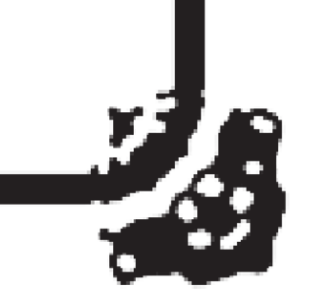
\includegraphics[width=0.4\textwidth]{image/introduction/inverse-design-bend.png}
  }

  % 2° row
  % Traditional splitter
  \subfigure[\emph{2--splitter} con diseño tradicional]{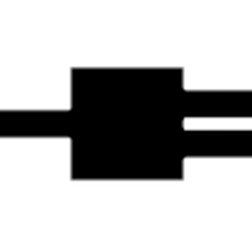
\includegraphics[width=0.4\textwidth]{image/introduction/traditional-splitter.png}}
  \hfill
  % Inverse design splitter
  \subfigure[\emph{2-splitter°} obtenido con diseño inverso. Extraído de \citep{Su2020}]{
    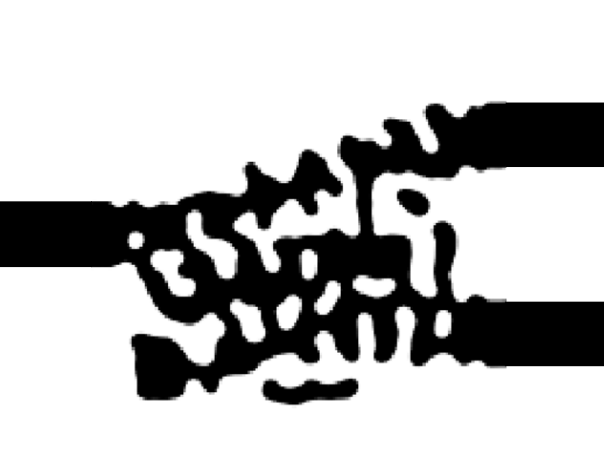
\includegraphics[width=0.4\textwidth]{image/introduction/inverse-design-splitter.png}
  }

  \caption{Diseños tradicionales y obtenidos a partir de diseño inverso de un \emph{bend-90°} y \emph{2-splitter}}
  \label{fig:devices}

\end{figure}

\section{Descripción del  Problema}


Para poder calcular las propiedades físicas de un dispositivo (e.g. campo eléctrico, transmitancia) se debe resolver las ecuaciones de Maxwell.
Así, con el objetivo de evaluar las propiedades de cualquier geometría se suele utilizar métodos numéricos como elementos finitos (FEM) y diferencias finitas en el dominio de tiempo (FDTD) \citep{Schneider2019}.
Con estos planteamientos se selecciona una región rectangular a optimizar y se la divide  en $n \times m$  píxeles como si fuera una imagen, ver Figure \ref{fig:bend-discretization}. 
Luego, a cada píxel se le asocia el número $0$ o $1$.
Típicamente, cero representa la presencia de $SiO_2$ en la ubicación del píxel y uno la presencia de $Si$ \citep{Molesky2018}.

\begin{figure}[h]
  \centering
  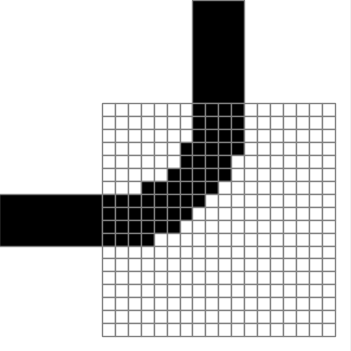
\includegraphics[scale=0.6]{image/introduction/bend-discretization.png}
  \caption{\emph{Bend-90} con una región de diseño discretizada en $18 \times 18$ píxeles. Cada píxel negro representa la presencia de $Si$ y cada píxel blanco de $SiO_2$}
  \label{fig:bend-discretization}
\end{figure}

El diseño inverso comienza definiendo los requerimientos del dispositivo para luego tratar de buscar entre los $2^{n \times m}$ posibles diseños algún candidato que se adapte a lo que se busca \citep{Su2020, Molesky2018}.
Como prueba de concepto, trabajos como el de \cite{Malheiros-Silveira2020} parametrizaron $2^{10 \times 10}$ posibles diseños.
Por otro lado, \cite{Su2020} con el objetivo de fabricar un dispositivo con buen rendimiento, configuró un espacio de búsqueda de $2^{34 \times 34}$ opciones.
Así, se presentan algunas dificultades con el diseño inverso:

\begin{enumerate}
  \item Es imposible evaluar todas los posibles diseños.
  \item Las simulaciones computacionales son muy costosas \citep{Kudyshev2020}.
  \item El espacio de búsqueda es altamente no convexo \citep{Su2018}.
  \item No todos los diseños son fabricables \citep{Su2020}.
  \item Cada dispositivo es una clase distinta de problema \citep{Molesky2018}.
\end{enumerate}


De este modo, existe una demanda crítica de un \emph{framework} capaz de optimizar dispositivos con un elevado número de parámetros dentro de un espacio de búsqueda no convexo \citep{Kudyshev2020}. Este es un problema muy grande, por ello en la presente tesis nos centraremos en optimizar un \emph{bend-90°} y un \emph{2-splitter}.

\section{Justificación}

Deste el punto de vista industrial, el \emph{bend-90°} y \emph{2-splitter} se han escogido debido a que han sido estudiados usando diseño inverso desde el 2004, pero aún no han encontrado aplicación masiva en la industria \citep{Molesky2018}. 

Desde el punto de vista computacional, este problema es interesante porque ya hay estrategias computacionales conocidas para resolverlo, desde algoritmos evolutivos \citep{Hansen2016} hasta redes neuronales \citep{Goodfellow2015} y \emph{depth learning} \citep{Malkiel2018}. 
Además, debido al alto costo computacional de las simulaciones \citep{Schneider2019}, el trabajo requiere de computación de alto desempeño.
Así, es probable que se pueda obtener buenos resultados en la investigación aplicando el conocimiento ya existente en computación.

\section{Objetivos}

\begin{itemize}

  \item Evaluar y comparar el rendimiento y la convergencia de algoritmos de optimización usadas para optimizar un \emph{bend-90°} y \emph{2-splitter} usando computación de alto rendimiento.

  \item Fabricar el diseño con mejor rendimiento que se obtenga del \emph{bend-90°} y del \emph{2-splitter} para poder comparar las simulacionales computacionales con las mediciones físicas.

%El siguiente objetivo es implementar un modelo de \emph{deep learning} que pueda predecir el \emph{performance} de un \emph{bend-90°} y de un \emph{2-splitter} con un error cuadrático medio menor a \leonidas{TODO: INVESTIGAR CUANTO DEBERÍA SER}. 

\end{itemize}



\section{Aportes}

Este trabajo busca brindar una comparativa de las técnicas de optimización más relevantes que se aplican para optimizar un \emph{bend-90°} y un \emph{2-splitter} cuando estos son parametrizados con un elevado número de variables.
